\chapter{Implementation}
\label{chapter:Chapter 4}
\lhead{Chapter 4. \emph{Implementation}}

In this Chapter, we present a description of the Implementation of \todo[inline]{need a framework name}. Firstly, we provide a Data Analysis from the provided Historical data, which \todo[inline]{needs way more talk}.

\section{Data Analysis}
\label{section: Data Analysis}
In order to gain insight and find the limitations of the AIS Data, we decided analyze the provided Historical AIS Data. For this Section, the Data Analysis we used the historical AIS Data-Set made publicly available by \cite{DATASET}.

Analysis of the provided Historical Data, was conducted by firstly analyzing the overall distribution of the Data-Set and after the analysis of each variable. 
The used Data-Set is composed of \textbf{18.684.115} AIS Messages originated by \textbf{4555} different Vessels. The Data-Set covers a Period of 6 Months (from 2015-10-01 to 2016-03-31), from a area nearby Brest, France represented in Figure \ref{fig:DS_Sample}.

\begin{figure}[H]
	\centering
	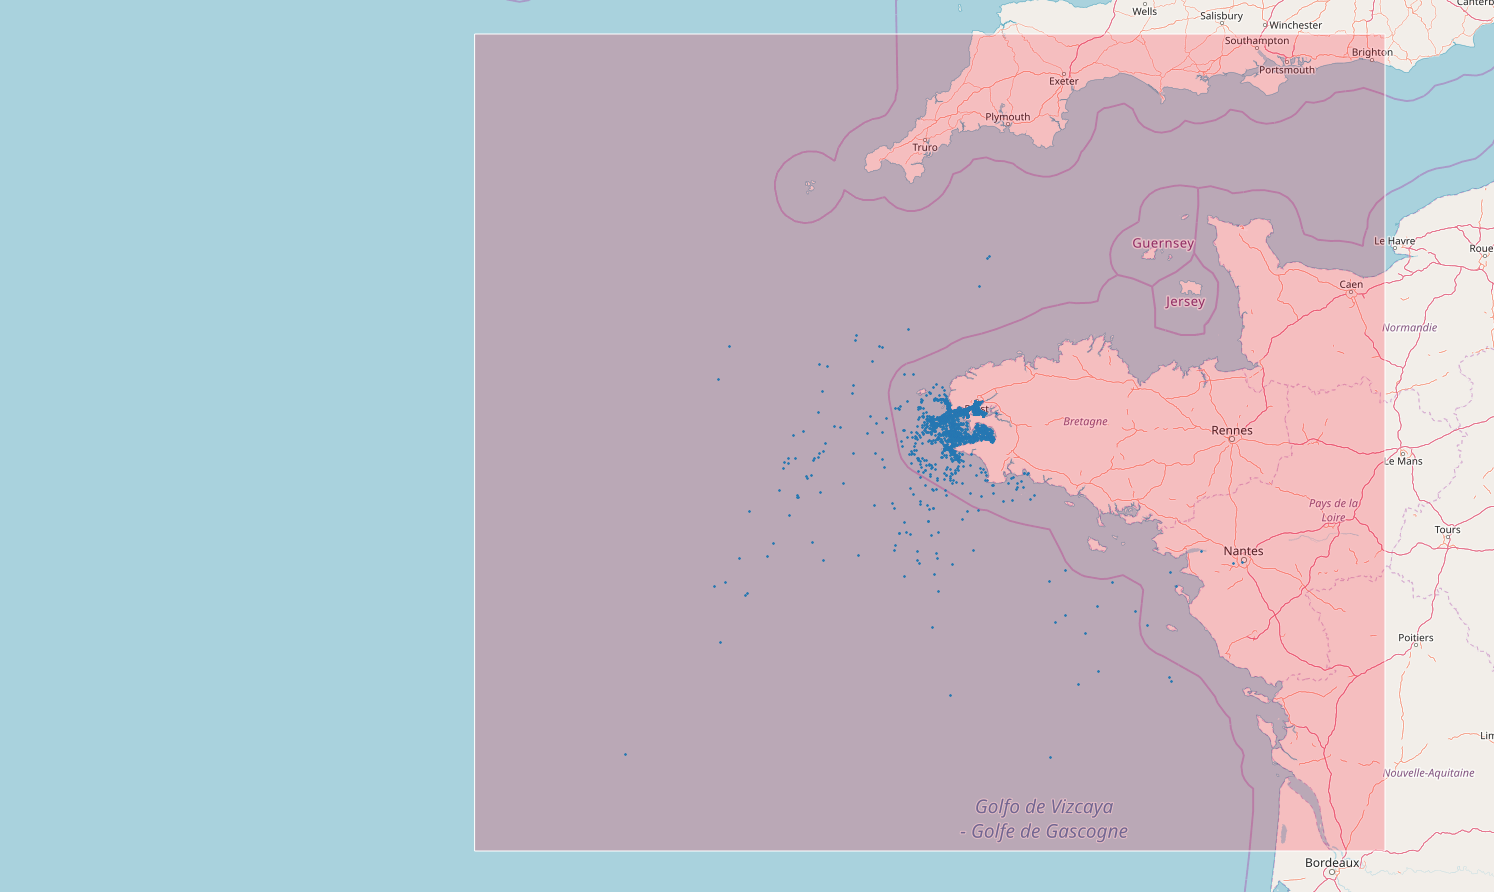
\includegraphics[scale = .23]{figures/Ch4/nari_DS_ex2.png}
    \caption{Area of the Data-Set represented in the Red, with a sample of 50.000 AIS Positions.}
    \label{fig:DS_Sample}
\end{figure}
Every AIS Message provided in the Data-Set, is composed by the features that derive from the AIS Dynamic Information. In Table \ref{Table: Data-Set Features}, we describe the Data-Set features and also the unit and range of each feature. 

\begin{table}[H]
\centering
\caption{My caption}
\label{Table: Data-Set Features}
\begin{tabular}{@{}llll@{}}
\toprule
Feature & Description                  & Unit               & Range          \\ \midrule
MMSI    & AIS Navigational Status.     &                    & 0 to 99999     \\
Status  & AIS Navigational Status.     &                    & 0 to 15        \\
Turn    & Rate of turn, right or left. & degrees per minute & 0 to 720       \\
SOG     & Speed Over Ground.           & knots              & 0 to 111*      \\
COG     & Course Over Ground.          & degrees            & 0º to 360º     \\
X       & Longitude.                   & degrees            & -180º to +180º \\
Y       & Latitude.                    & degrees            & -90º to 90º    \\
Time    & received Time-Stamp.         & Unix Time          &                \\ \bottomrule
\end{tabular}
\end{table}

With the same Data-Set it is possible to enrich the AIS Dynamic messages, with the Vessels Static information. By interpolating the MMSI we can gain information of the actual Vessels Static information, which represents the actual Vessel Characteristics, such as the dimensions of the Vessel, and what had more importance for us the Vessel Type.
Vessel Type, is a classification system, where each Vessel is categorized by the type of activities it preforms. The Vessel Type, is represented by a number from 0 to 99, where the first digit represents the general category of the subject vessel, and the combination of the first digit with the second represent a specific activity of the Vessel. In Table XX we present the Vessel General category associated with the first digit, and also the specific Categories which are more representative in the Data-Set.

\begin{table}[H]
\centering
\caption{My caption}
\label{my-label}
\begin{tabular}{@{}llll@{}}
\toprule
First Digit & General Category & Relevant Categories &                                                                                         \\ \midrule
1           & Reserved         &                     &                                                                                         \\
2           & Wing In Ground   &                     &                                                                                         \\
3           & Special Category & 30 - Fishing        & 30 - 286(6\%)                                                                           \\
4           & High-Speed Craft &                     &                                                                                         \\
5           & Special Category &                     &                                                                                         \\
6           & Passenger        &                     &                                                                                         \\
7           & Cargo            & 70 - Cargo          & \begin{tabular}[c]{@{}l@{}}70 - 1511(33\%)\\ 79 - 273(6\%)\\ 71 - 217(5\%)\end{tabular} \\
8           & Tanker           & 80 - Tanker         & 80 - 342(7\%)                                                                           \\
9           & Other            &                     & 99 - 1192(26\%)                                                                         \\ \bottomrule
\end{tabular}
\end{table}




posiextrapolate Vessels Static information, thus gaining information of the Vessel Characteristics, such as, the dimension characteristics of the Vessel and the Vessel type information. Vessel Type is a good indicator to filter the Data, based on the Vessel data thus knowing if

effective way, to query the Dtafilter the Vessel activities based on the Vessel type.
represented in Table, is significant to gain information by know in

\section{Data Cleaning}
As any 

\todo[inline]{MORE TEXT HERE} The features represented above, were al contained 

\section{Trajectory Definition}
In this Section we present our definition our interpretation and formulation of Vessel Trajectory, 
Representing a Vessel Trajectory data, can become a difficulty in the Maritime domain. Currently there are a vast number of solutions described in the literature, presenting different solutions for different types of problems. 

Our approach to represent a Maritime trajectory, was to consider a trajectory as a whole, this is, as Vessel are obliged to broadcast their AIS information in a semi-continuous rates; knowing that each AIS broadcast message represent the instantaneous kinematic information from a Single Vessel, aggregating this information over time will represent a Vessel Trajectory. 

Thus, by identifying each vessel by its unique identifier (MMSI), the trajectory can be considered as the set of AIS messages, identified by the MMSI of each Vessel.

\begin{figure}[H]
	\centering
	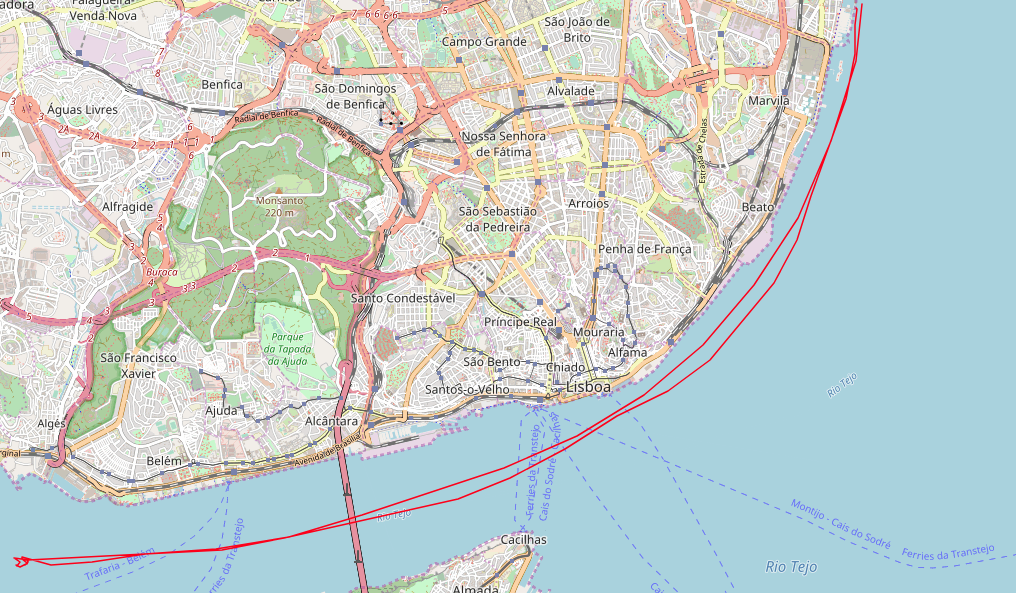
\includegraphics[scale = .3]{figures/Ch3/traj_example.png}
    \caption{Trajectory snapshot(2017-11-05 10:22 to 2017-11-05 22:42) from Vessel MMSI: 255806006}
    \label{fig: TrajectorySMM_example}
\end{figure}

Although, as each AIS message is time-stamped(contains the time in which was broadcast), our representation of trajectory can be defined as Multivariate Time-Series, this is for each trajectory we have $N$ time-series, in which $N$ represents the number of features considered for each trajectory, further explained in the subsections bellow.

\subsection{Multivariate Time-Series Analogy}
As mentioned above, each Trajectory is considered as a Time Series composed of Multiple features.  

in Fig. \ref{fig: MTimeSeries_example}, we represent the Vessel trajectory showend in figure X. 
For each trajectory we consider the features representing 
main features that a which in order to normalize our analysis of a Vessel Route, we ...
\todo[inline]{TODO dar palha para introduzir esta imagem}

\begin{figure}[H]
	\centering
	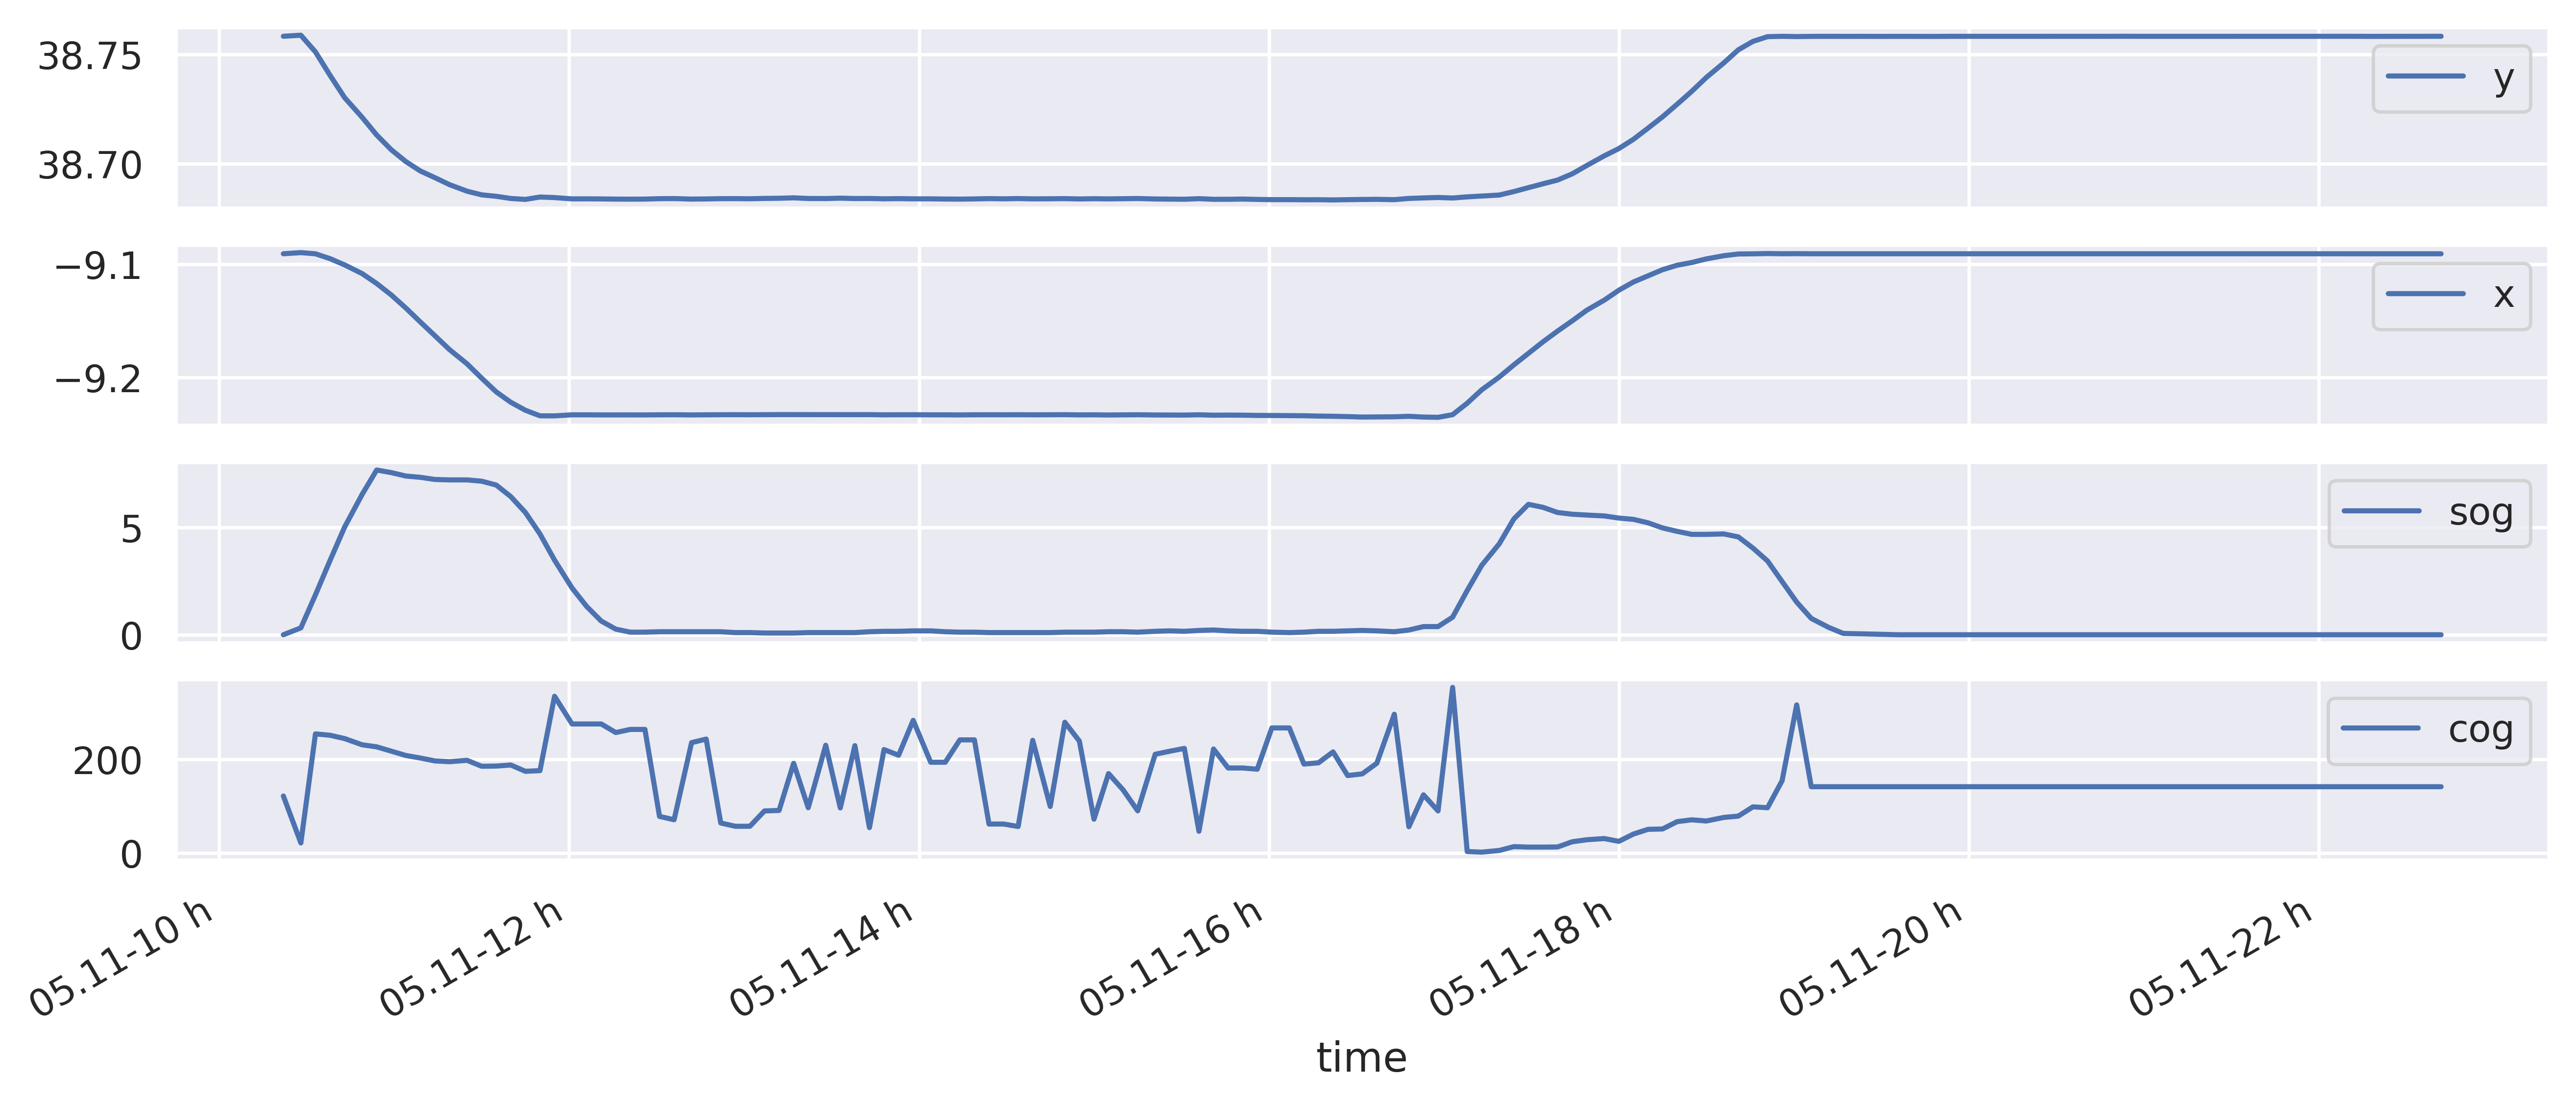
\includegraphics[scale = .5]{figures/Ch3/ts_example.png}
    \caption{Trajectory represented in Fig.X, presented as a Multivariate Time Series.}
    \label{fig: MTimeSeries_example}
\end{figure}

\todo[inline]{Needs Intro for this section...}

\section{Feature Engineering}
\subsection{Latitude Longitude Normalization}
In order to normalize the reported AIS positions, either from the AIS streams or the used Data-Set, we defined a set number of decimal cases used. This is done as most of AIS providers only assure a GPS precision of 0.0001 minutes accuracy, but what we found was that some reported positions come with up to 8 decimal cases, which can be caused just from how the Data-Set files were written.

So our normalization process, was to assure that every Vessel position was normalized to a precision on 4 decimal cases; as it represents a global position precision of 11m to 4m, as it is shown in Table \ref{Table: Degree Precision}.

\begin{table}[H]
\centering
\caption{Degree precision versus the approximate radius of measured error.}
\label{Table: Degree Precision}
\begin{tabular}{lrrrr}
\hline
\multicolumn{1}{c}{\begin{tabular}[c]{@{}c@{}}Decimal \\ Places\end{tabular}} & \multicolumn{1}{c}{Degrees} & \multicolumn{1}{c}{\begin{tabular}[c]{@{}c@{}}Precision \\ Equator\end{tabular}} & \multicolumn{1}{c}{\begin{tabular}[c]{@{}c@{}}Precision \\ 45º N/S\end{tabular}} & \multicolumn{1}{c}{\begin{tabular}[c]{@{}c@{}}Precision \\ 67º N/S\end{tabular}} \\ \hline
0 & 1.0 & 111.3Km & 78.7Km & 43.5Km \\
1 & 0.1 & 11.3Km & 7.8Km & 4.4Km \\
2 & 0.01 & 1.13Km & 787.1m & 435m \\
3 & 0.001 & 111.3m & 78.7m & 43.5m \\
4 & 0.0001 & 11.3m & 7.8m & 4.4m \\
5 & 0.00001 & 1.3m & 0.7m & 0.4m \\ \hline
\end{tabular}
\end{table}

\todo[inline]{Geohash - https://en.wikipedia.org/wiki/Geohash}



\subsection{Distance to Coast}
The Distance to Shore influences, the navigational behaviour for some type of Vessels. In order to enrich the features used in our Anomaly Detection methods it seemed necessary to extrapolate the Distance to Shore for every point in the Data-Set. Although in order to calculate the Distance to Shore over the whole data-set, and in real time to streams of AIS data it is mandatory to represent the Coastline in a efficient manner. 
For this we used the ocean coastline data\footnote{http://www.naturalearthdata.com}, which represented the Global Ocean Coast line in a vector of \textbf{547.503} points, which is equivalent of representing in a 1:10m scale.

The calculation of the closest point was done with a Nearest Neighbor approach, using the Ball Tree algorithm. The choice of this algorithm was done, due to the high volume of data we were using, and the possibility of using the Haversine Distance measures \eqref{eq: Haversine} in the already implemented methods from \todo{http://scikit-learn.org/stable/modules/generated/sklearn.neighbors.BallTree.html}.

Haversine is a distance metric commonly used in Vessel Navigation, it is commonly used as both Latitude and Longitude features are represented in a spherical coordinate system. $d_({p_1}, {p_2})$ represents the distance between the 2 point $p1(lat_1, lon_1)$ and $p2(lat_2, lon_2)$, and where $r$ represents the approximate radius of the Earth which we considered \textbf{6.367.000m} in our experiments.

\begin{equation}
d = 2r sin ^{-1} (\sqrt{sin^2(\frac{lat_{2}-lat_{1}}{2})+cos(lat_{1})cos(lat_{2})sin^2(\frac{long_{2}-long_{1}}{2}))}
\label{eq: Haversine}
\end{equation}

\subsubsection{Distance to Port}
Do i want to talk about this? Linear is not a good aproximation.

\subsection{Stopped/Moving}
Enriching the reported Vessel Kinematics by determining if whether a Vessel is Moving or Stopped represents a information gain on overall Vessel Trajectory that can be addressed, for the understanding of the normal Vessels Behaviour itself and even further, the possible detection of Anomalies.
Thus, the approaches we used to classify every Vessel transmission as Stopped or Moving is shown in the following subsections:

\textbf{Rule Based Approach}:
This approach is vastly used in the literature, as it is the simplest way to characterize the stopping of a Vessel, based solely on the Speed or as reported in the AIS the Speed Over Ground (SOG). Thus, Vessels Positions that have a Speed under a certain defined threshold $\Delta$ are considered as Stopped and the opposite are considered Moving, as it is shown in equation \ref{eq: MovingRule}, where $p_n$ represents actual point we want to the point which we want to c.
\begin{equation}
kinematic status(p_n) = \left\{\begin{matrix}
p_n.SOG > \Delta; & Moving\\ 
p_n.SOG \leq  \Delta; & Stopped
\end{matrix}\right.
\label{eq: MovingRule}
\end{equation}

The most commonly used value, found in the literature for $\Delta$ was 0.5 knots, which was also the Threshold we initially tested for, but we found that this leads to the miss-labeling of effectively Positions that are Moving, more specifically Fishing Vessels that due to their type of fishing activities, greatly slow their Speed for short periods of Time, which cannot be labeled as Stopped.
\todo[inline]{Need intro to this image}
\missingfigure{Trajectory of a Shipping Vessel that is considered as stopped.}

In order to mitigate the problem described above we used a \textbf{Rolling Mean}, which is a common method for Time Series Analysis in countless different fields.  By Smoothing the Vessels Speed Feature, we reduce the random or abrupt variations in the observed Speed features,  thus better describing the normal kinematic, stopping  pattern of a Vessel. 
\todo[inline]{Need intro to this image}
\missingfigure{Trajectory of a Shipping Vessel that is considered as stopped then with the rolling mean!}

\section{Anomaly Detection Service}

\subsection{Navigational Status Validation}
AIS Navigational Status describes the Vessel current navigational activity based on a set static set of defined Status, as shown in Table XX. The Navigational Status needs to be manually set and constantly updated (according to the current Vessel activity), by the Vessel crew members. The problem with relying on Human action to update the actual Vessel Navigational Status is that is really prone to errors. 

\begin{table}[H]
\centering
\caption{My caption}
\label{my-label}
\begin{tabular}{@{}cl@{}}
\toprule
\begin{tabular}[c]{@{}c@{}}Navigational \\ Status Value\end{tabular} & \multicolumn{1}{c}{Description} \\ \midrule
0 & under way using engine \\
1 & at anchor \\
2 & not under command \\
3 & restricted maneuverability \\
4 & constrained by draught \\
5 & moored \\
6 & aground \\
7 & engaged in fishing \\
8 & under way sailing \\
9 - 14 & reserved for future use \\
15 & Default \\ \bottomrule
\end{tabular}
\end{table}

Our approach towards the detection of the miss-use Navigational Status, started by firstly analyzing what each Navigational Status was used for, and the frequency of which was used. We concluded, based on the frequency count of each Status that there are AIS Status which are solely used in special scenarios. Thus, for this we focus on the detection and validation of AIS Status that can be justified on the Vessels Dynamic Features.

and represent little occurrences on the global count of the Data-Set.

as it is represented in Fig

being considered Anomalous, our approach towards the detection of this  









